\documentclass[12pt]{article}

\usepackage{mathtools}
\usepackage{cancel}
\usepackage{amsmath}
\usepackage{amsthm}
\usepackage{amsfonts}
\usepackage{amssymb}
\usepackage{enumerate}
\usepackage{graphicx}\usepackage{mdframed}
\usepackage{multicol}
\usepackage{verbatim}
\usepackage{tikz}
\usepackage{braket}
\usepackage[T1]{fontenc}
\usetikzlibrary{automata,chains,arrows,positioning,calc}
\usepackage[margin = .7in]{geometry}
\geometry{letterpaper}
\linespread{1.2}

%% One of the nicest things about LaTeX is you can create custom macros. If  there is a long-ish expression that you will write often, it is nice to give it a shorter command.
%% For our common number systems.
\newcommand{\R}{\mathbb{R}} %% The blackboard-bold R that you have seen used for real numbers is typeset by $\mathbb{R}$. This macro means that $\RR$ will yield the same result, and is much shorter to type.
\newcommand{\N}{\mathbb{N}}
\newcommand{\Z}{\mathbb{Z}} 
\newcommand{\Q}{\mathbb{Q}}
\newcommand{\E}{\mathbb{E}}
\newcommand{\C}{\mathbb{C}}
\newcommand{\Lbb}{\mathbb{L}}
\newcommand{\Prob}{\mathbb{P}}
\newcommand{\Afancy}{\mathcal{A}}
\newcommand{\Bfancy}{\mathcal{B}}
\newcommand{\Cfancy}{\mathcal{C}}
\newcommand{\Dfancy}{\mathcal{D}}
\newcommand{\Efancy}{\mathcal{E}}
\newcommand{\Ffancy}{\mathcal{F}}
\newcommand{\Gfancy}{\mathcal{G}}
\newcommand{\Hfancy}{\mathcal{H}}
\newcommand{\Ifancy}{\mathcal{I}}
\newcommand{\Jfancy}{\mathcal{J}}
\newcommand{\Kfancy}{\mathcal{K}}
\newcommand{\Lfancy}{\mathcal{L}}
\newcommand{\Mfancy}{\mathcal{M}}
\newcommand{\Nfancy}{\mathcal{N}}
\newcommand{\Ofancy}{\mathcal{O}}
\newcommand{\Pfancy}{\mathcal{P}}
\newcommand{\Qfancy}{\mathcal{Q}}
\newcommand{\Rfancy}{\mathcal{R}}
\newcommand{\Sfancy}{\mathcal{S}}
\newcommand{\Tfancy}{\mathcal{T}}
\newcommand{\Ufancy}{\mathcal{U}}
\newcommand{\Vfancy}{\mathcal{V}}
\newcommand{\Wfancy}{\mathcal{W}}
\newcommand{\Xfancy}{\mathcal{X}}
\newcommand{\Yfancy}{\mathcal{Y}}
\newcommand{\Zfancy}{\mathcal{Z}}
\renewcommand{\thempfootnote}{\arabic{mpfootnote}}

\newcommand{\var}{\text{var}}
\newcommand{\cov}{\text{cov}}

\newcommand{\argmin}{\text{arg}\,\text{min}}
\newcommand{\indep}{\perp \!\!\! \perp}


%% Your macros can even accept arguments. 
\newcommand\abs[1]{\left| #1 \right|} %% This will do the same but with vertical bars. I.e., \abs{STUFF} gives |STUFF|
\newcommand\parens[1]{\left( #1 \right)} %% Similar. \parens{STUFF} gives (STUFF)
\newcommand\brac[1]{\left[ #1 \right]} %% Similar. \brac{STUFF} gives [STUFF]
\newcommand\solution[1]{\begin{mdframed}
\emph{Solution.} #1
\end{mdframed}}
\newcommand\solutionproof[1]{\begin{mdframed}
\begin{proof} #1
\end{proof}
\end{mdframed}}

\begin{document}
\noindent Jonathan Pei \hfill Date

\begin{center}
  {\large CS 285 Homework 1: Imitation Learning}
\end{center}

\section{Analysis}

\begin{enumerate}
    \item Let us define 
    \[\Pr[\mathrm{mistake}] \coloneqq \Pr[\text{make a mistake at some time step $\leq t$}].\]

    Then, following the same idea as in lecture we have 
    \begin{align*}
      p_{\pi_\theta}(s_t) &= (1 - \Pr[\mathrm{mistake}]) \cdot p_{\pi^*}(s_t) + \Pr[\mathrm{mistake}] \cdot p_{\mathrm{mistake}}(s_t) \\
      \implies \sum_{s_t} \abs{p_{\pi_\theta}(s_t) - p_{\pi^*}(s_t)} &= \Pr[\text{mistake}] \cdot \sum_{s_t} \abs{p_{\text{mistake}}(s_t) - p_{\pi^*}(s_t)} \\
      &\leq 2 \Pr[\text{mistake}]
    \end{align*}

    Now, it suffices to show that $\Pr[\text{mistake}] \leq T \epsilon$:
    \begin{align*}
      \Pr[\text{mistake}] &= \Pr\left(\cup_{0 \leq i \leq t} \text{ first mistake occurs at time step $i$}\right) \\
      &\leq \sum_{i \leq t}\Pr\left(\text{first mistake at time step $i$}\right) \\
      &= \sum_{i \leq t}\Pr\left(\text{matches expert policy until time step $i$}\right) \\
      &\leq \sum_{i \leq t} \sum_{s_i} \Pr[\text{make a mistake at $s_i$}] \cdot p_{\pi^*}(s_i) \\
      &= \sum_{i \leq t} \E_{p_{\pi^*}(s_i)}[\pi_\theta (a_i \neq \pi^*(s_i) \mid s_i)] \\
      &\leq \sum_{i \leq T} \E_{p_{\pi^*}(s_i)}[\pi_\theta (a_i \neq \pi^*(s_i) \mid s_i)] \\
      &\leq T \epsilon
    \end{align*}
    as desired. Note that we applied the union bound between the 1st and 2nd lines.

    \item \begin{enumerate}
      \item When the reward only depends on the last state, we have 
      \begin{align*}
        J(\pi^*) - J(\pi_\theta) &= \sum_{t=1}^T \E_{p_{\pi^*}(s_t)}[r(s_t)] - \sum_{t=1}^T \E_{p_{\pi_\theta}(s_t)}[r(s_t)] \\
        &= \E_{p_{\pi^*}(s_T)}[r(s_T)] - \E_{p_{\pi_\theta}(s_T)}[r(s_T)] \\
        &= \sum_{s_T} r(s_T) \cdot p_{\pi^*}(s_T) - \sum_{s_T} r(s_T) \cdot p_{\pi_\theta}(s_T) \\
        &\leq R_{\mathrm{max}} \cdot \sum_{s_T} \abs{p_{\pi_\theta}(s_T) - p_{\pi^*}(s_T)} \\
        &\leq 2R_{\mathrm{max}} \cdot T \epsilon \\
        &= \mathcal{O}(T\epsilon )
      \end{align*}

      \item For any arbitrary reward, we have 
      \begin{align*}
        J(\pi^*) - J(\pi_\theta) &= \sum_{t=1}^T \E_{p_{\pi^*}(s_t)}[r(s_t)] - \sum_{t=1}^T \E_{p_{\pi_\theta}(s_t)}[r(s_t)] \\
        &= \sum_{t=1}^T \sum_{s_t} r(s_t) \cdot (p_{\pi^*}(s_t) - p_{\pi_\theta}(s_t)) \\
        &\leq R_{\mathrm{max}}\sum_{t=1}^T \sum_{s_t} \abs{p_{\pi_\theta}(s_t) - p_{\pi^*}(s_t)} \\
        &\leq R_{\mathrm{max}} \sum_{t=1}^T 2T\epsilon \\
        &= 2R_{\mathrm{max}} \cdot T^2 \epsilon \\
        &= \mathcal{O}(T^2 \epsilon)
      \end{align*}
    \end{enumerate}
\end{enumerate}

\newpage

\section{Behavioral Cloning}

\begin{enumerate}
  \item I report the mean and standard deviation of my policy's return (over multiple rollouts) on the Ant and Walker2d tasks:
  \begin{table}[h!]
    \begin{center}
    \begin{tabular}{|c|c|c|}
      \hline
      Task & \texttt{Eval\_AverageReturn} & \texttt{Eval\_StdReturn} \\
      \hline
      Ant & 3876.619 & 1213.65 \\ 
      Walker2d & 651.389 & 909.57 \\
      \hline
    \end{tabular}
    \caption{\textbf{Evaluation Mean and Standard Deviation of my policy's return over multiple rollouts, on the Ant and Walker2d tasks.}
    I set \texttt{seed} to 4, \texttt{ep\_len} to 1000, and \texttt{eval\_batch\_size} to 10000. All other hyperparameters (e.g. model architecture, learning rate, etc.) are identical and the default values.
    We observe very different results for the Ant and HalfCheetah tasks, even though the training configurations used were the exact same. In particular, our policy was able to achieve 81.2\% of the performance of the expert on the Ant task, and only 12.1\% on the Walker2d task.}
  \end{center}
  \end{table}

  \item I experimented with varying the number of hidden layers in the MLP model, on the Walker2d task. A graph is provided below:
  \begin{figure}[h!]
    \begin{center}
    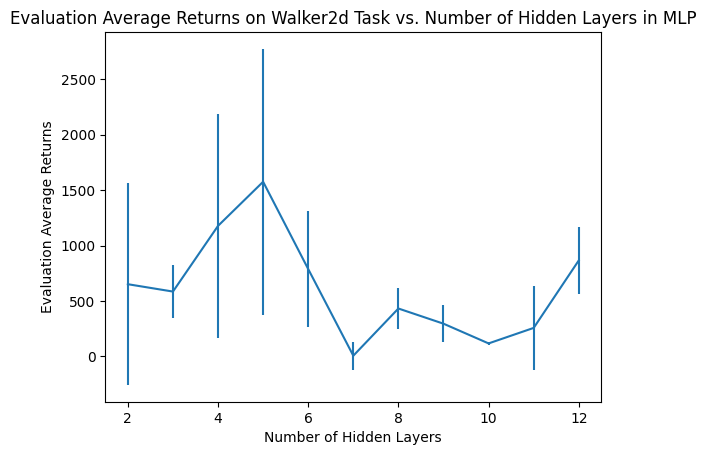
\includegraphics[width=\textwidth*2/3]{walker2d_hidden.png}
    \caption{\textbf{Evaluation Average Returns on the Walker2d task vs. Number of MLP Hidden Layers.} I varied the hidden layer from 2 to 12, and kept all other training configurations the same as in part (1). We can see that the agent's performance increases until it peaks at around 5 hidden layers, after which it mostly decreases until 12 layers. I wanted to try adjusting the number of hidden layers because deeper neural networks are capable of learning more complex patterns, until a certain point where they begin to overfit. My experiment (roughly) exhibits this behavior.}
  \end{center}
  \end{figure}
\end{enumerate}

\section{\textsc{DAgger}}

\begin{itemize}
  \item [2.] After running DAgger on the Ant and Walker2d tasks, I present the following two graphs:
  \begin{figure}[h!]
    \begin{center}
    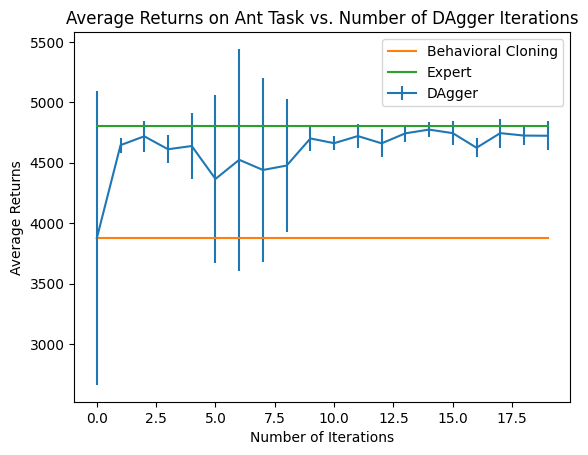
\includegraphics[width=\textwidth*2/3]{ant_dagger.png}

    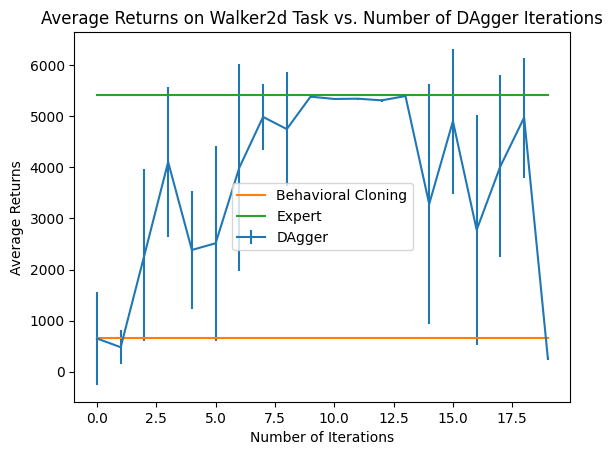
\includegraphics[width=\textwidth*2/3]{walker2d_dagger.png}
  \end{center}
  \caption{\textbf{Average Returns on Ant and Walker2d Tasks vs. Number of DAgger Iterations.} I ran the agent on the Ant and Walker2d tasks, with the same configurations as described in the previous section. We see that DAgger substantially outperforms behavioral cloning, especially in Walker2d.}
  \end{figure}
\end{itemize}

\section{Discussion}

\begin{enumerate}
  \item I spent 2 hours on Q1, 6 hours on Q3, and 2 hours on Q4.
  \item Nope.
\end{enumerate}


\end{document}